\section{Data processing}

\subsection{Noise averaging}

\begin{minipage}{0.52\linewidth}

\begin{figure}[H]
    \centering
    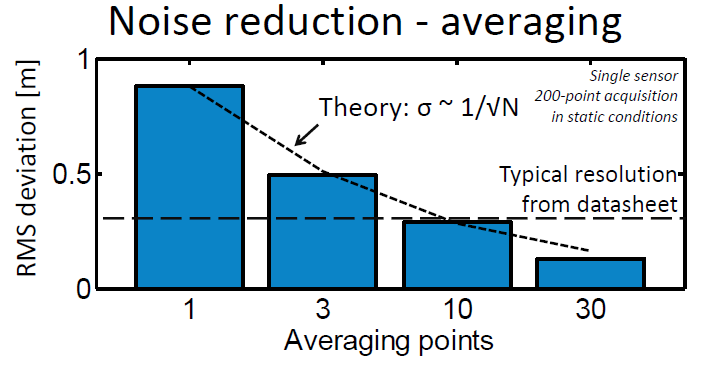
\includegraphics[width = \textwidth]{L6/img/averaging.PNG}
\end{figure}

\end{minipage}\hfill
\begin{minipage}{0.45\linewidth}
Block averaging can be used to reduce the random
intrinsic noise. RMS deviation ($\sigma$) ultimately limited by other effects. Simple post-processing as averaging with decimation
(downsampling) saves data bandwidth/memory
space but leads to loss of temporal resolution.
\end{minipage}

\subsection{Digital filtering}

Intrinsic thermal noise is reduced thanks to band-pass filter. 
Crosstalk noise/interference is reduced thanks to band-reject filters.
Environmental noise is better eliminated with periodic calibration or ratiometric sensing.

\vspace{0.2cm}
\begin{minipage}{0.45\linewidth}

\begin{itemize}
    \item Digital filters
    \begin{itemize}
        \item Powerful : better filtering performances
        \item Theory and data limited
    \end{itemize}
\end{itemize}

\end{minipage}\hfill
\begin{minipage}{0.45\linewidth}

\begin{itemize}
    \item Analog filters
    \begin{itemize}
        \item Cheap (no MCU = microcontroller)
        \item Component limited
    \end{itemize}
\end{itemize}
\end{minipage}

\vspace{0.2cm}
\textbf{Why are analog filters needed ? }
The instrumentation amplifier amplifies the DC component so we need a high-pass filter to limit this DC component which came from the ambient light (environmental noise). A low pass filter is also needed before data acquisition to eliminate the high frequency noise.

\subsubsection{Band-pass and band-reject filters}

With $h_1[n]$ and $h_2[n]$ the low-pass and a high-pass impulse responses respectively, we have the following expressions for the band-pass ($h_1[n]$ and $h_2[n]$ in series) and band-reject ($h_1[n]$ and $h_2[n]$ in parallel) filters:

\begin{minipage}{0.45\linewidth}
\begin{figure}[H]
    \centering
    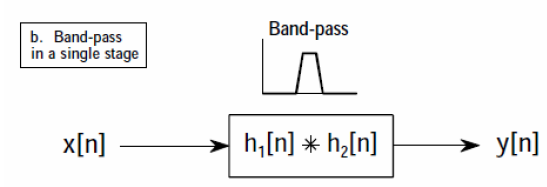
\includegraphics[width = \textwidth]{L6/img/band-pass.PNG}
\end{figure}
\end{minipage}\hfill
\begin{minipage}{0.45\linewidth}
\begin{figure}[H]
    \centering
    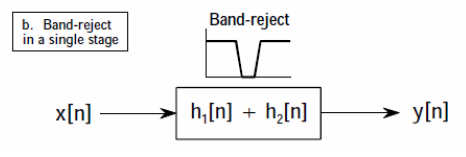
\includegraphics[width = \textwidth]{L6/img/band-reject.PNG}
\end{figure}
\end{minipage}


\subsubsection{Digital filters performances}

\begin{minipage}{0.45 \linewidth}
\paragraph{Frequency domain}
\begin{itemize}
    \item Roll-off (short
    transition band) = steepness of the transition for raised cosine filter.
    \item Flat passband
    \item Stopband
    attenuation
\end{itemize}
\end{minipage}\hfill
\begin{minipage}{0.45 \linewidth}
\paragraph{Time domain}

\begin{itemize}
    \item Step response
    \item No overshoot
    \item Linear phase
\end{itemize}

\end{minipage}

\vspace{0.5cm}

In both case, we have to take care of the computational complexity of the digital filter. 

\subsubsection{Digital filter classification}

\begin{mydef}
    Finite Impulse Response (FIR) filters only use the input samples
to produce an output sample $\rightarrow$ \textbf{high performances}
\end{mydef}

\begin{mydef}
    Infinite Impulse Response (IIR) filters use both the input samples and the previous output
sample to produce an output sample $\rightarrow$ use the output feedback $\rightarrow$ \textbf{fast and low-power} (low computational complexity)
\end{mydef}
Generally, filters can be implemented in the digital domain based on FIR or IIR. But there is always a trade-off between filter performances (roll-off, step response, \dots) and computational complexity.

\begin{figure}[H]
    \centering
    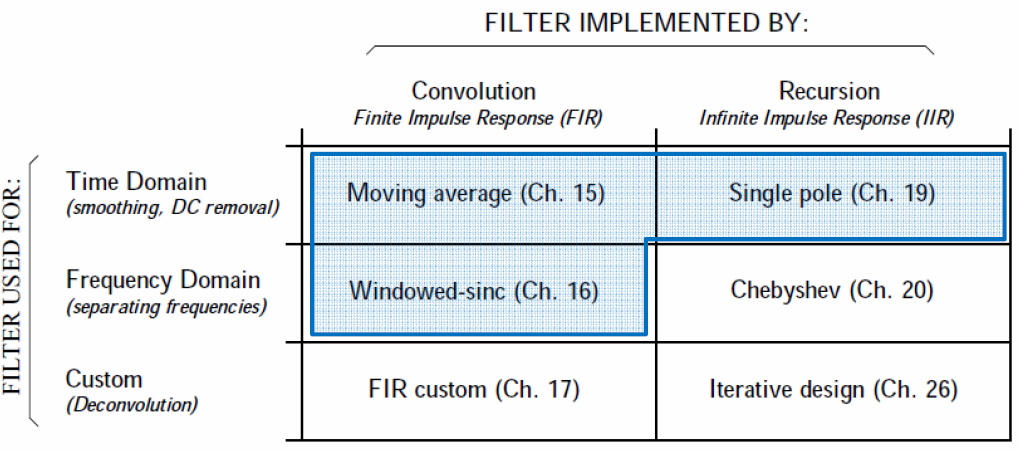
\includegraphics[width = 0.7\textwidth]{L6/img/classification.PNG}
\end{figure}

\subsubsection{Moving-average FIR}

\begin{minipage}{0.5 \linewidth}

This filter consists of a simple convolution with
a rectangle of unity area in the time domain. The results in the frequency domain is then a multiplication with a sinc function.
It limits white random noise
while preserving fast response $\rightarrow$ good smoothing filter. It has a poor frequency roll-off
and stopband attenuation $\rightarrow$ poor low-pass filter.

We can improve frequency-domain performances
with multiple-pass moving-average FIR (in series) at
the expense of more computation complexity.

Moving average better captures the signal dynamics than a simple average.

The computation complexity can be reduced with recursive implementation.
\end{minipage}\hfill
\begin{minipage}{0.5 \linewidth}

\begin{figure}[H]
    \centering
    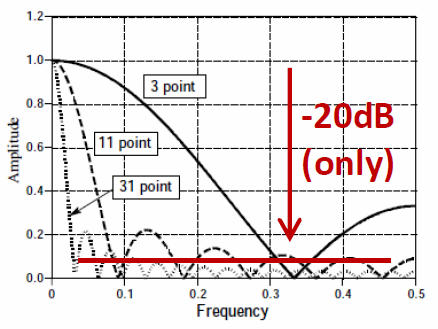
\includegraphics[width = 0.7\textwidth]{L6/img/moving-area.PNG}
\end{figure}

\end{minipage}

\subsubsection{Windowed-sinc FIR}

\begin{minipage}{0.5 \linewidth}

\begin{figure}[H]
    \centering
    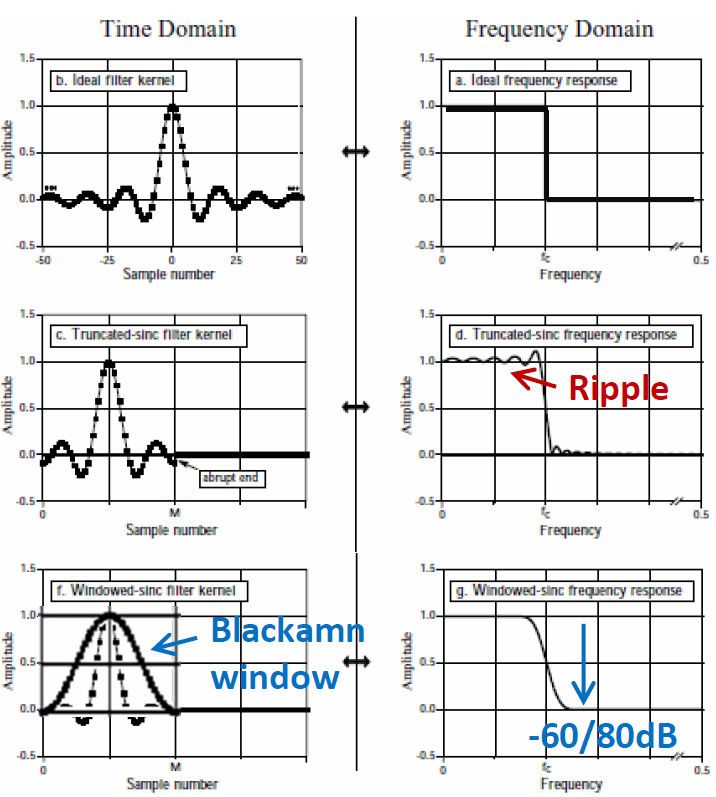
\includegraphics[width = \textwidth]{L6/img/sinc-FIR.PNG}
\end{figure}

\end{minipage}\hfill
\begin{minipage}{0.5 \linewidth}
The ideal low-pass
filter has a sinc
(sin(x)/x, sinus cardinal) impulse
response. To overcome the infinite range of the sinc function,
proper windowing is required with a Blackman or Hamming window.
\end{minipage}


\subsubsection{Single pole IIR}

\begin{minipage}{0.5 \linewidth}
The single pole IIR has a low computational complexity
(re-use of previous outputs). It requires a floating-point
representation to avoid overflow or underflow errors. Excellent smoothness compared to moving average FIR.

\end{minipage}\hfill
\begin{minipage}{0.5 \linewidth}

\begin{figure}[H]
    \centering
    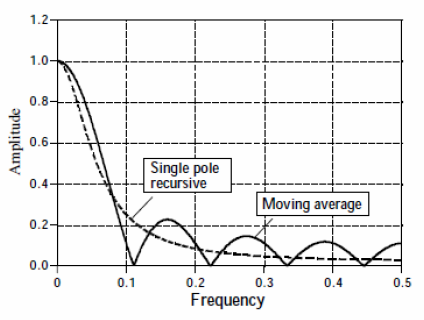
\includegraphics[width = \textwidth]{L6/img/single-pole.PNG}
\end{figure}

\end{minipage}

If we want steeper step response, \textbf{oversampling} is required.

\subsubsection{Oversampling}

\begin{minipage}{0.5 \linewidth}
Oversampling allows to reduce noise (quantization noise) while preserving
dynamic characteristics. We see that using big oversampling coupled with digital filtering gives best performances.

However, oversampling is limited by
\begin{itemize}
    \item data storage (non-volatile memory = cost)
    \item battery capacity (limited power consumption)
\end{itemize}


\end{minipage}\hfill
\begin{minipage}{0.5 \linewidth}
\begin{figure}[H]
    \centering
    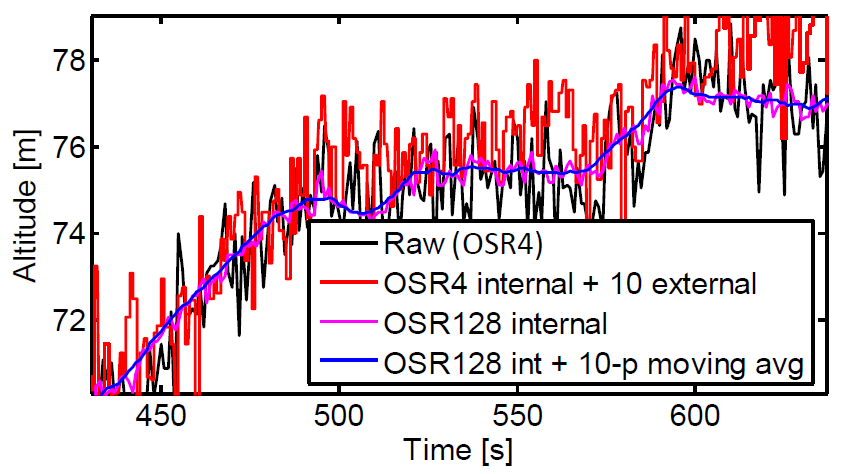
\includegraphics[width = 0.8\textwidth]{L6/img/digital-oversampling.PNG}
\end{figure}

\end{minipage}

\subsubsection{Analog vs Digital filters}

\begin{minipage}{0.5 \linewidth}
Digital filters have better
performances but
\begin{itemize}
\item they have a frequency
dynamic range limited
by the number of points
processed at once
(computational
complexity),
\item they have an amplitude
dynamic range limited
by the ADC resolution,
\item they require a CPU/MCU.
\end{itemize}
\end{minipage}\hfill
\begin{minipage}{0.5 \linewidth}
\begin{figure}[H]
    \centering
    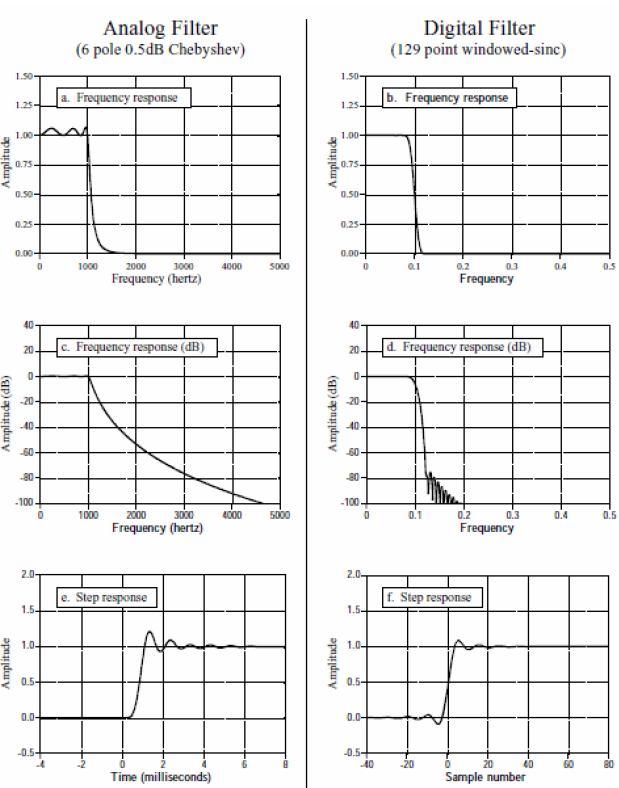
\includegraphics[width = 0.6\textwidth]{L6/img/analogvsdigital.PNG}
\end{figure}
\end{minipage}


\subsubsection{Summary}

Good data acquisition and processing requires prior
knowledge of the input stimulus to acquire and the
sensor producing the output signal.
\begin{itemize}
\item Device-to-Device variations $\rightarrow$ calibration
\item Intrinsic noise $\rightarrow$ digital filtering (with oversampling)
\item Crosstallk noise $\rightarrow$ digital filtering
\item Environmental noise $\rightarrow$ analog filtering / system solutions
(differential/ratiometric sensing, periodic calibration)
\end{itemize}

Basic signal processing tasks can be done:
\begin{itemize}
\item Off-line or real-time post-process (Matlab/Labview)
\item MCU to save memory footprint/communication rate
\item Most sensors today come with embedded data processing
functions to offload the MCU $\rightarrow$ perform the task directly on the sensors.
\end{itemize}
